\chapter{Theory}
\label{chap:theory}

\chapterquote{Eat, sleep, rave, repeat}
{Fatboy Slim}

\section{The standard model of particle physics}
\label{sec:sm}

% \begin{figure}
%   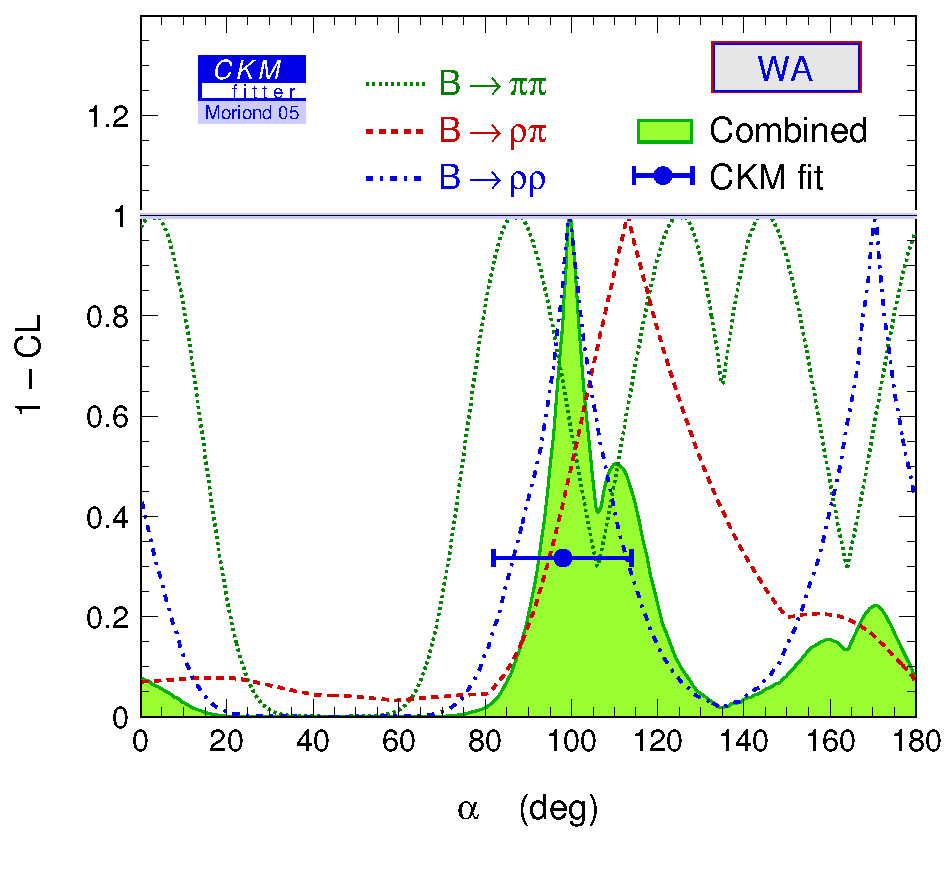
\includegraphics[width=\largefigwidth]{ckmfitter-alpha-combined}
%   \caption[CKM Fitter constraints on \alphaCKM.]%
%   {CKM Fitter constraints on \alphaCKM from combined \BToPiPi,
%     \BToRhoPi and \BToRhoRho decay analyses.}
%   \label{fig:CKMFitter}
% \end{figure}

\section{Supersymmetry}
\label{sec:susy}

% \begin{sidewaysfigure}
%   \begin{center}
%   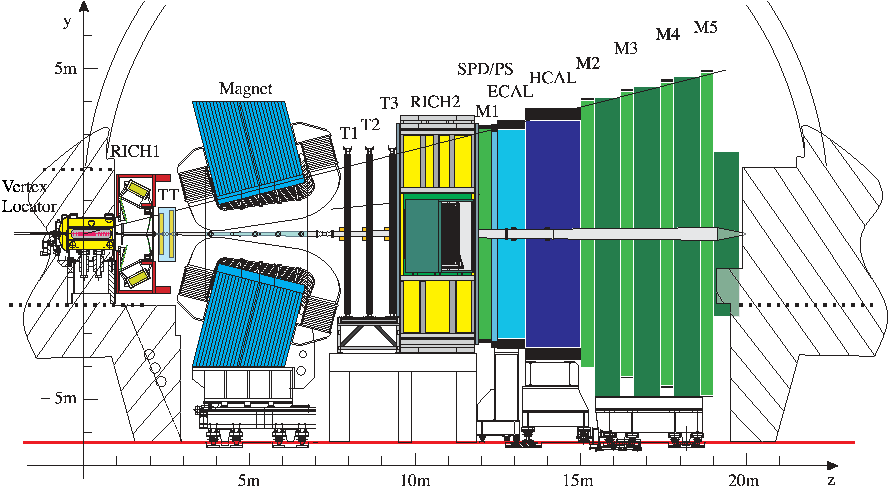
\includegraphics[width=0.8\textheight]{figs/example/lhcb-detector-cross-section}
%   \caption[Cross-section view of \LHCb, cut in the non-bending $y$--$z$ plane]%
%     {Cross-section view of \LHCb, cut in the non-bending $y$--$z$ plane.}
%   \label{fig:LHCbCrossSection}
%   \end{center}
% \end{sidewaysfigure}

\section{Signatures of supersymmetry at the \LHC}

Decays etc.
